\documentclass[10pt,a4paper]{article}
\usepackage[utf8]{inputenc}
\usepackage[italian]{babel}
\usepackage{amsmath}
\usepackage{amsfonts}
\usepackage{amssymb}
\usepackage{graphicx}
\usepackage[left=2cm,right=2cm,top=2cm,bottom=2cm]{geometry}
\newcommand{\rem}[1]{[\emph{#1}]}

\author{Gruppo AC \\ Federico Belliardo, Francesco Mazzoncini, Giulia Franchi}
\title{Esercitazione N.3: Misure DC su transistor e NOT TTL.}
\begin{document}

\maketitle
\section{Scopo e strumentazione}
Verificare il funzionamento del transistor npn come amplificatore in un circuito in DC, determinando il guadagno in corrente continua ed analizzare l'uso del transistor in un circuito logico NOT. Nell'esperienza ci si servirà di uno stabilizzatore di tensione $LM785$ e di un potenziometro (\textit{trimmer}).

\section{Identificazione dei terminali dei componenti}

\paragraph{Misura della polarità delle giunzioni del diodo}
Per prima cosa abbiamo analizzando le polarità delle giunzioni del transistor, verificando che si trattasse effettivamente  di un diodo npn (abbiamo ottenuto valori positivi per le giunzioni BC e BE).

\paragraph{Misura delle resistenze del trimmer}

Utilizzando il multimetro digitale abbiamo misurato le resistenze del trimmer: ai suoi estremi la resistenza è risultata costante $R_{tot}= (102.7 \pm 0.8)\, k\Omega$, mentre la resistenza tra il terminale intermedio e uno dei due estremi è risultata variabile. Prendendo l'uscita dalla parte delle scritte sul case la resistenza aumenta in senso orario.

\paragraph{Controllo dello stabilizzatore di tensione}
Abbiamo montato il circuito in  figura \ref{circuito} verificando che  la $V_{out}$ rimanesse costante a $V_{out} = (5.00 \pm 0.03) \, V$ (misurata con multimetro digitale) variando $V{in}$ da $6V$ a circa $20V$. 

\section{Misure in DC sul transistor}

Si sono misurati i valori dei componeni utilizzati: $R_L = (0.977 \pm 0.008) \, k\Omega$ e $R_B= (46.7 \pm 0.4) \, k\Omega $ e $C=(9.8 \pm 0.4) \, nF$
La tensione dell'alimentatore è stata misurata essere: $V_1 = (10.06 \pm 0.06) \, V$. 

\begin{figure}[!htb]
  \centering
  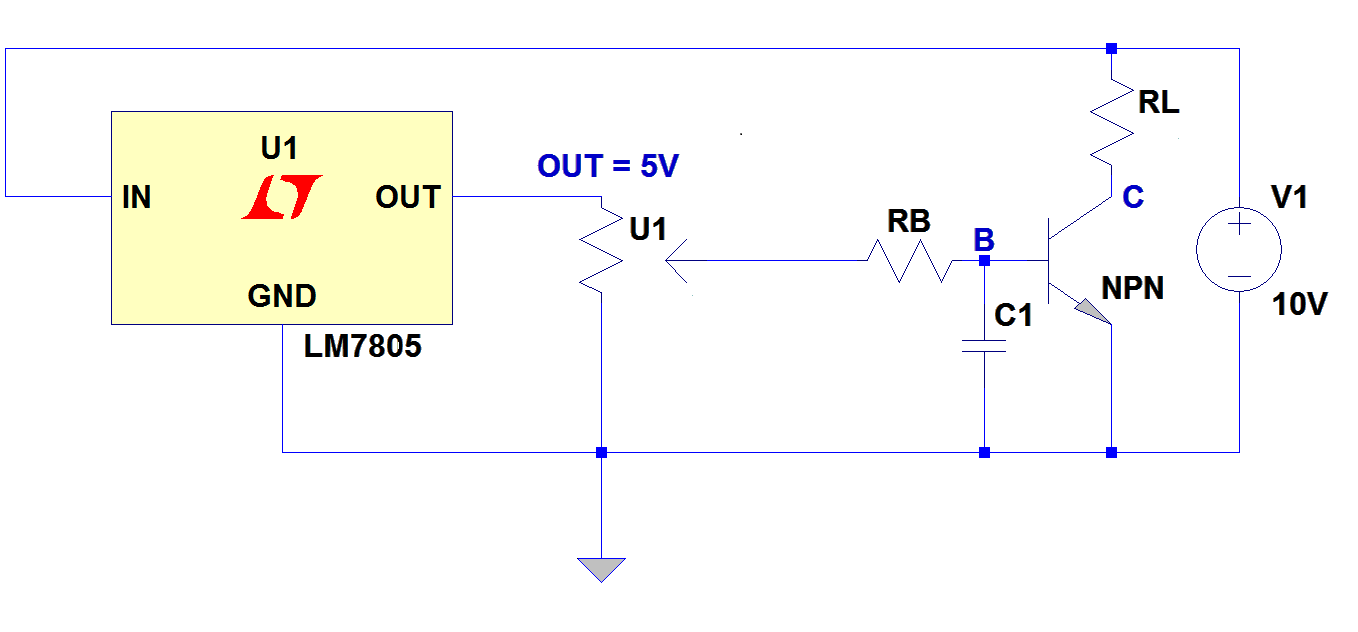
\includegraphics[scale=0.4]{circuito}
\caption{Circuito di amplificazione di correnti continue}
\label{circuito}
\end{figure}

\paragraph{Calcolo della retta di carico}
La retta di carico teorica ($I_C = \frac{V_1 - V_{CE}}{R_L}$) è stata disegnata come retta tra due punti (a $I_c = 0$ e a $V_{ce} = 0$) sul grafico delle curve cartteristiche del transistor, come si vede nella figura
 \ref{caricoTeorica}.
 
\begin{figure}[!htb]
  \centering
  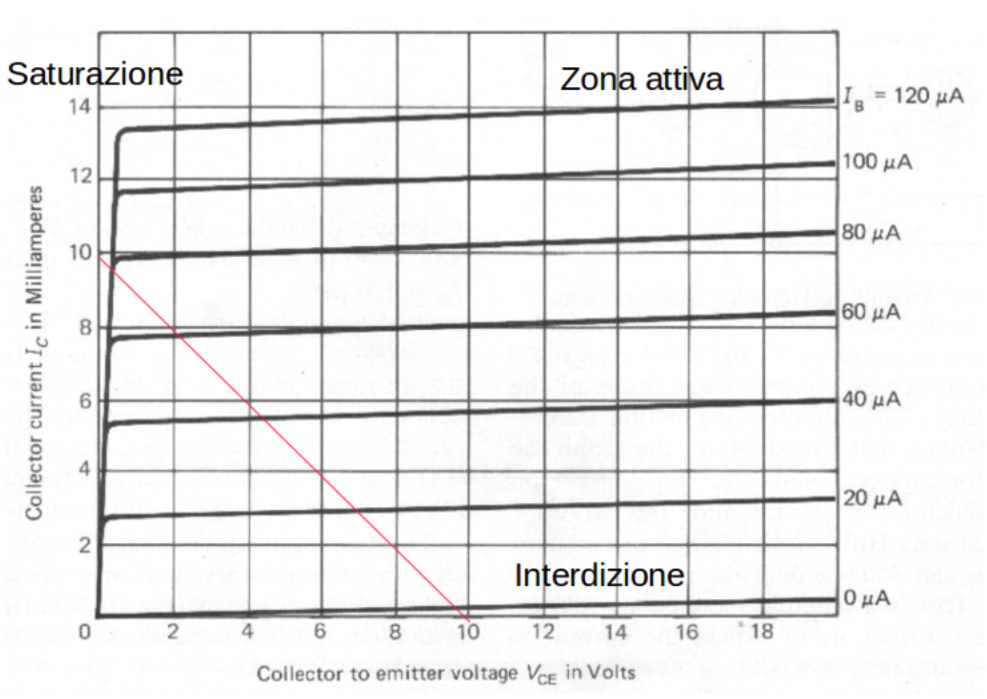
\includegraphics[scale=0.4]{rettaCarico.png} 
\caption{Circuito di amplificazione di correnti continue} \label{caricoTeorica}
\end{figure}
 
\paragraph{Misure sul circuito.}

Abbiamo collegato il multimetro digitale in parallelo alla resistenza $R_B$ e i due canali dell'oscilloscopio ai terminali B e C del transistor. In questo modo siamo stati in grado di misurare contemporaneamente la caduta di tensione $V_{R_B}$ ai capi della resistenza $R_B$, $V_{BE}$ e $V_{CE}$.\\
Abbiamo preso varie misure variando la resistenza del potenziometro (ruotando quindi la vite di regolazione). Grazie alle relazioni $I_B = V_{R_B}/R_B$ e $I_C = \frac{V_1-V_{CE}}{R_L}$ abbiamo potuto calcolare la corrente $I_B$ in ingresso alla base e la corrente del collettore $I_C$.\\
Il canale 1 è collegato alla base e il canale 2 è collegato al collettore.
Abbiamo riportato tutte le misure nella tabella \ref{misureDC}.

\begin{table}[!htb]\centering
\begin{tabular}{|c|c|c|c|c|c|}
\hline
$V_{rb}$ & $\sigma V_{rb}$ & $V_{ce}$ & $\sigma V_{ce}$ & $\sigma V_{be}$ & $\sigma V_{be}$\\
\hline
4.16 & 0.02 & 0.32 & 0.01 & 0.88 & 0.03\\
3.97 & 0.02 & 0.300 & 0.009 & 0.86 & 0.03\\
3.22 & 0.02 & 0.31 & 0.01 & 0.84 & 0.03\\
2.92 & 0.02 & 0.31 & 0.02 & 0.86 & 0.03\\
0.0033 & 0.0003 & 10.0 & 0.3 & 0.076 & 0.003\\
3.26 & 0.02 & 0.200 & 0.007 & 0.74 & 0.02\\
2.88 & 0.02 & 0.240 & 0.007 & 0.74 & 0.02\\
2.55 & 0.02 & 0.216 & 0.007 & 0.74 & 0.02\\
2.36 & 0.02 & 0.228 & 0.007 & 0.74 & 0.02\\
2.06 & 0.01 & 0.260 & 0.008 & 0.74 & 0.02\\
1.49 & 0.01 & 2.24 & 0.07 & 0.72 & 0.02\\
1.34 & 0.01 & 3.0 & 0.1 & 0.70 & 0.02\\
1.13 & 0.01 & 4.2 & 0.1 & 0.70 & 0.02\\
0.963 & 0.005 & 5.0 & 0.2 & 0.68 & 0.02\\
0.744 & 0.004 & 6.2 & 0.2 & 0.66 & 0.02\\
0.545 & 0.003 & 7.3 & 0.2 & 0.64 & 0.02\\
0.406 & 0.002 & 8.2 & 0.3 & 0.64 & 0.02\\
0.229 & 0.002 & 9.0 & 0.3 & 0.64 & 0.02\\
0.0243 & 0.0002 & 10.0 & 0.3 & 0.50 & 0.02\\
0.0135 & 0.0001 & 10.0 & 0.3 & 0.296 & 0.009\\
0.0038 & 0.0001 & 10.0 & 0.3 & 0.084 & 0.003\\
0.0084 & 0.0001 & 10.0 & 0.3 & 0.184 & 0.006\\
0.0065 & 0.0001 & 10.0 & 0.3 & 0.140 & 0.005\\
0.0051 & 0.0001 & 10.0 & 0.3 & 0.112 & 0.004\\
\hline
\end{tabular}
\caption{Misure sul transistor in DC} \label{misureDC}
\end{table}

\begin{figure}[!htb]
  \centering
  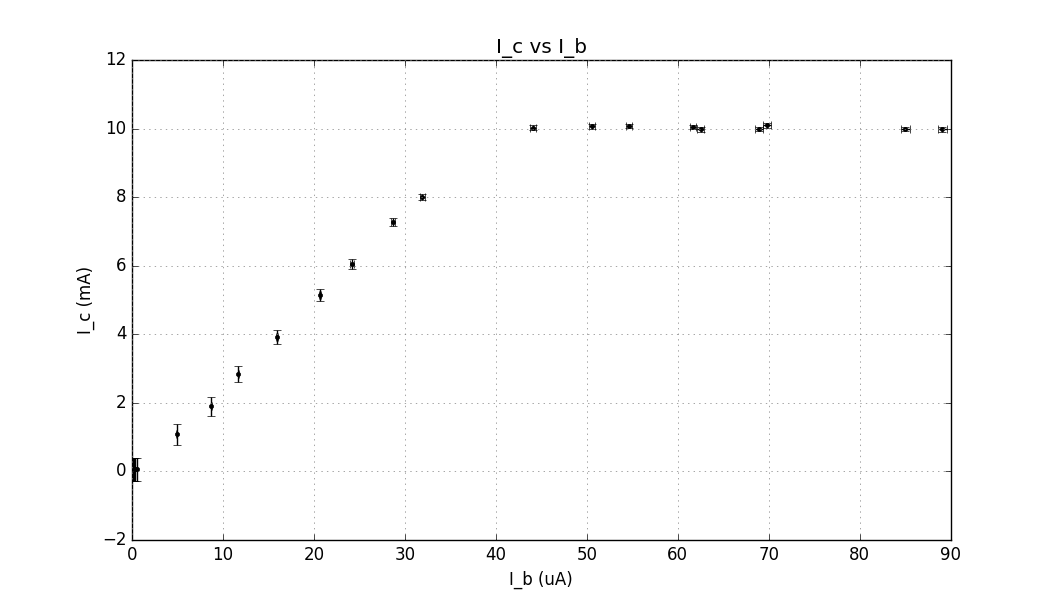
\includegraphics[scale=0.5]{IcIb.png} 
\caption{Corrente di collettore vs. Corrente di base}  \label{IcIb}
\end{figure}

\begin{figure}[!htb]
  \centering
  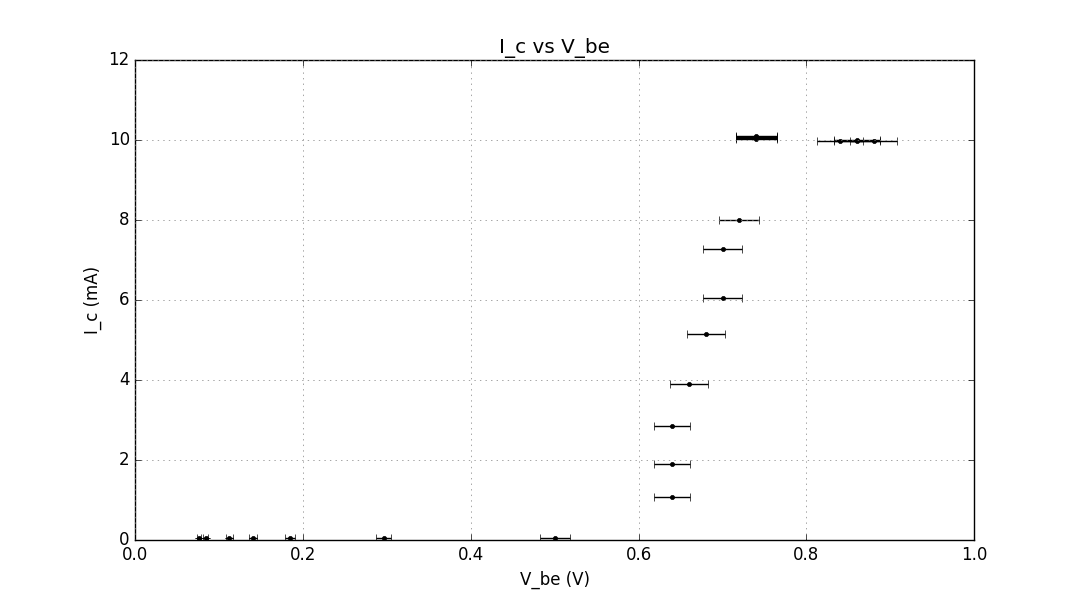
\includegraphics[scale=0.5]{IcVbe.png} 
\caption{Corrente di collettore vs. Tensione di base}  \label{IcVbe}
\end{figure}

Nei grafici \ref{IcIb} e \ref{IcVbe} gli errori sono riportati propagando l'incertazza sistematica sulle misure di tensione dell'oscilloscopio. Nei fit successvi questa incertezz non è stata tenuta in considerazione (non come si può vedere dal fatto che i $\chi^2$ ottenuti sono ragionevoli).


\paragraph{Corrente di saturazione.}
La massima corrente di collettore erogabile dal transistor è determinata dall'equazione di Kirchoff relativa alla maglia destra del circuito  $V_1 = R_LI_C + V_{CE}$, quindi il massimo valore di $I_C$ si ha per il minimo valore di $V_{CE}$ ($V_{sat}$), che è una caratteristica del transistor.\\
Si è eseguto un fit di una costante ($\chi^2 = 4.5/7$) per trovare la corrente di saturazione ottenendo il valore $I = (10.03 \pm 0.03) \, mA$. Grafico in figura \ref{saturazione}. Da questo valore si ottiene una tensione di saturazione $V_{sat} = (0.26 \pm 0.10) \, V$. Il manuale del transistor riporta l'indicazione che la tensione di saturazione è $V_{ce} < 0.5 \, V$, in accordo con qaunto trovato.

\begin{figure}[!htb]
  \centering
  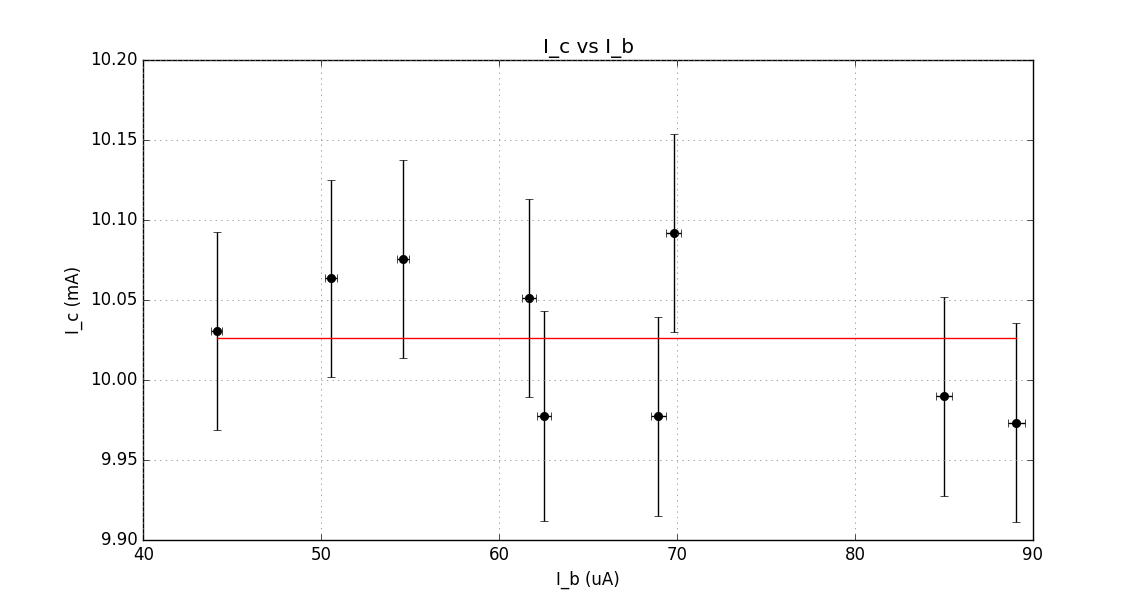
\includegraphics[scale=0.5]{fitSaturazione.png} 
\caption{Corrente di collettore vs. Tensione di base} \label{saturazione}
\end{figure}

%(array([ 0.2597147 , -0.21176614]), array([[  6.41851612e-05,  -1.31426841e-03],
%      [ -1.31426841e-03,   3.13037663e-02]]))
%Chisquare/ndof = 0.566115/6
%('p = ', 0.99693848309662825)

\paragraph{Misura della costante di guadagno $h_{FE}$.}
Abbiamo calcolato il guadagno del transistor eseguendo un fit lineare di $I_C$ e $I_B$ con la  relazione $I_C=h_{FE}I_B+q$.
Dai dati della regione attiva riusciamo a stimare il guadagno del transistor, eseguendo il fit lineare (\ref{guadagno}) otteniamo il valore $h_{FE} = (260 \pm 8)$. Il fit ($\chi^2 = 0.6/6$) è stato applicato con unità di misura $mA$ e $\mu A$ sulle ordinate e sulle ascisse rispettivamente, questo mi da:
$a = (0.259 \pm 0.008)$, $b = (-0.2 \pm 0.2)$, la matrice di covarianza è: $\left(
\begin{array}{cc}
6.42 \cdot 10^{-5} & -1.31 \cdot 10^{-3} \\ 
-1.31 \cdot 10^{-3} & 3.13 \cdot 10^{-2}
\end{array}   
\right)$.
Il manuale del trasistor riporta: $100 < h_{FE} < 300$, in accordo con quanto misurato.

\begin{figure}[!htb]
  \centering
  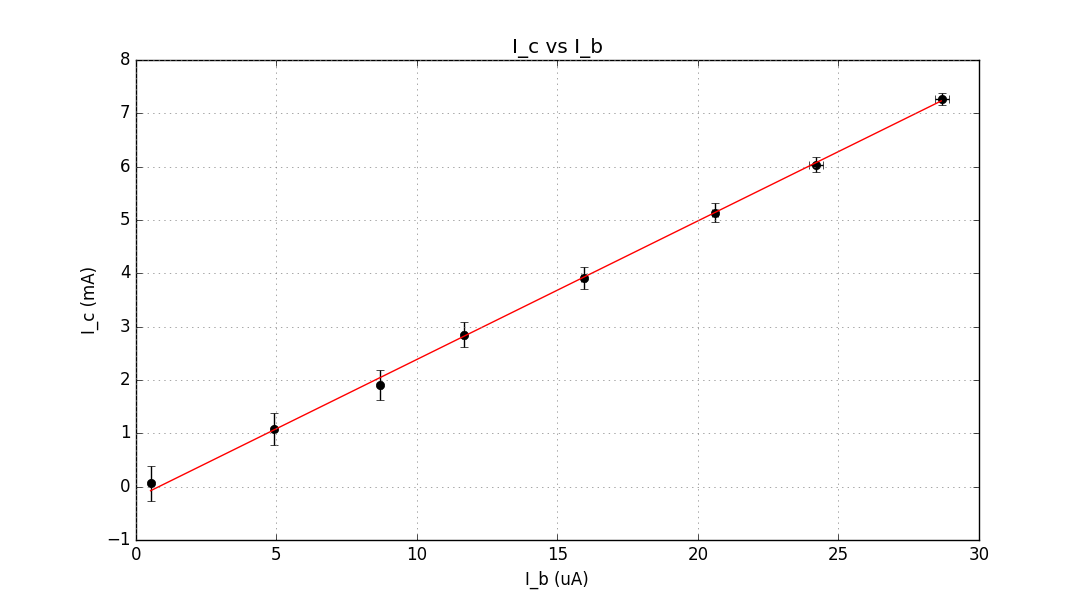
\includegraphics[scale=0.5]{rettaGuadagno.png} 
\caption{Corrente di collettore vs. Corrente di base} \label{guadagno}
\end{figure}

\paragraph{Variazione della retta di carico al variare della tensione di alimentazione.}
 
Abbiamo ruotato la vite regolatrice del trimmer resistivo finchè non si è ottenuto $V_{CE}\simeq 5V$ per una tensione di alimentazione di $V_1 = 10 \, V$. Si fissa il valore corrispondente della corrente $I_B$. Misuriamo  $V_{R_L}$ ai capi di $R_L$ con il multimetro digitale  e $V_{CE}$ tramite l'oscilloscopio al variare di $V_1$ tra $6\,V$ e $16\,V$. Tali dati sono riportati in tabella \ref{dati2}.

\begin{table}[!htb]\centering
\begin{tabular}{|c|c|c|c|c|c|}
\hline
$V_l$ & $\sigma V_l$ & $V_{ce}$ & $\sigma V_{ce}$\\
\hline
4.99 & 0.03 & 1.48 & 0.08\\
5.02 & 0.03 & 1.80 & 0.08\\
5.07 & 0.03 & 2.20 & 0.08\\
5.06 & 0.03 & 2.56 & 0.08\\
5.09 & 0.03 & 3.08 & 0.08\\
5.13 & 0.03 & 4.20 & 0.08\\
5.14 & 0.03 & 4.56 & 0.08\\
5.17 & 0.03 & 4.96 & 0.08\\
5.19 & 0.03 & 7.48 & 0.08\\
5.23 & 0.03 & 8.16 & 0.08\\
5.26 & 0.03 & 9.60 & 0.08\\
5.27 & 0.03 & 10.30 & 0.08\\
5.34 & 0.03 & 11.90 & 0.08\\
5.45 & 0.03 & 15.20 & 0.08\\
\hline
\end{tabular}
\caption{Tensione di Early}
\label{dati2}
\end{table}

Per gli intervalli di tensione che possiamo utilizzare (per mantenere funzionante lo stabilizzatore ($V_{1}  > 6 \, V$)) non riusciamo a misurare nessun dato nella zona di saturazione ma si osserva marcatamente l'effetto Early, come si vede in figura \ref{early}. Abbiamo tentato di determinare con un fit la tensione di Early.

\begin{figure}[!htb]
  \centering
  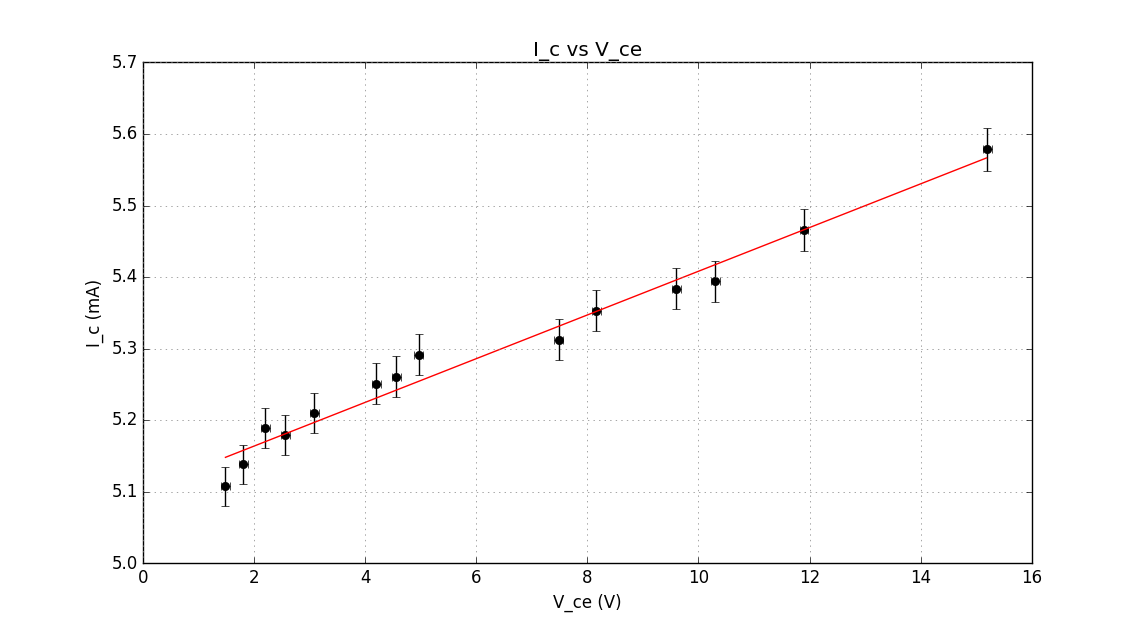
\includegraphics[scale=0.5]{Early.png} 
\caption{Effetto Early} \label{early}
\end{figure}

I parametri della retta fittata ($\chi^2 = 7.4/12$)  sono: $a = (3.1 \pm 0.2) \cdot 10^{-5} \frac{A}{V}$ e $b = (5.10 \pm 0.01)\, mA$. La matrice di covarianza dei paramentri è: $\left( 
\begin{array}{cc}
3.50\cdot 10^{-5} & -2.13\cdot 10^{-11} \\ 
-2.13\cdot 10^{-11} & 1.87 \cdot 10^{-10}
\end{array} \right)$.
Da questi dati si può stimare: $V_{Early} = (0.17 \pm 0.01) \, kV$.


 
\section{Uso del transistor in un circuito logico NOT }
\paragraph{Montaggio del circuito.}
Abbiamo montato il circuito rappresentato in  figura \ref{circuito2}.

\begin{figure}[!htb]
  \centering
  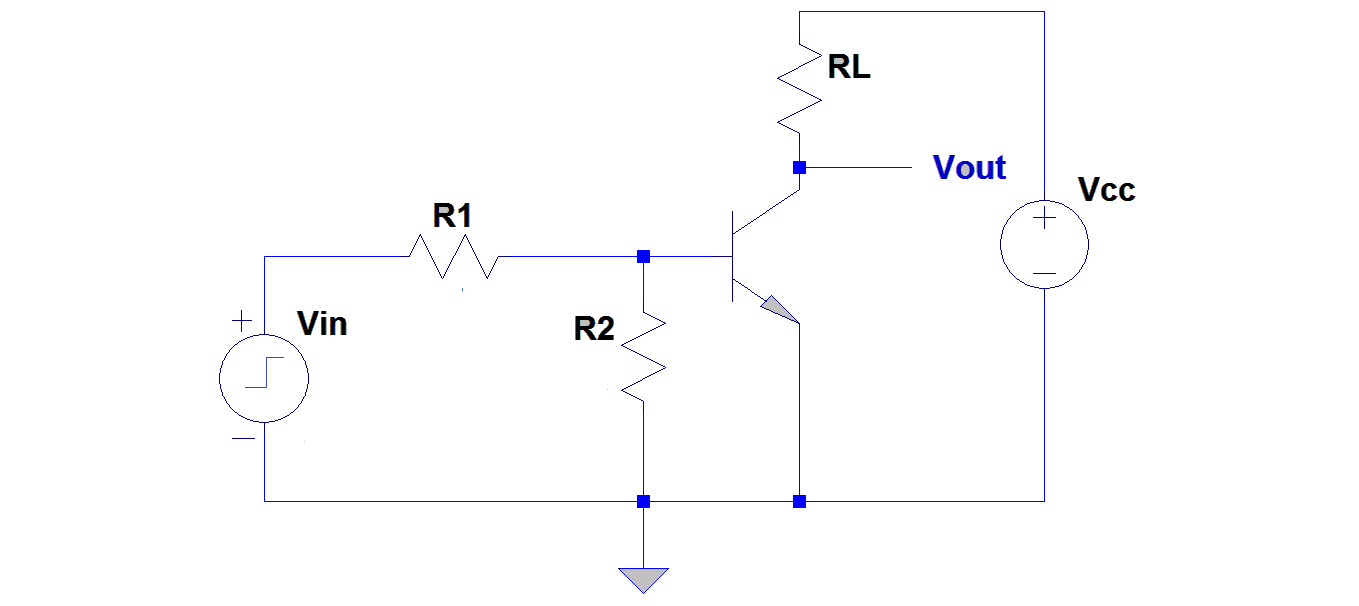
\includegraphics[scale=0.4]{circuito2} 
\caption{Circuito logico NOT.} \label{circuito2}
\end{figure} 

In ingresso abbiamo collegato  il generatore di funzioni in modalità output pulse, il quale genera un’onda quadra oscillante tra $0 V$ e $5 V$. Abbiamo usato  il generatore di tensione insieme allo stabilizzatore di tensione per ottenere  $V_{cc} = (5.00 \pm 0.03)$. \\ 
Questa configurazione permette di far funzionare il transistor in regime di saturazione e di interdizione al variare di $V_{in}$. Le resistenze usate ( misurate con un multimetro digitale ) sono : $R_1=(14.6 \pm 0.2) \, k\Omega$, $R_2=(100 \pm 1) k\Omega$ e $R_L=(2.1 \pm 0.1) k\Omega$.
Il generatore si segnali fornisce un'onda quadra a circa $7.5 Hz$.

\paragraph{Verifica del corretto funzionamento del circuito.}
Si sono misurate le tensioni di base e di collettore nei due regimi in cui $V_{in} = 0 \, V$ e $V_{out} = 5 \, V$ le misure sno riportate nella tabella \ref{voltNot}.

\begin{table}[!htb]\centering
\begin{tabular}{|c|c|c|}
\hline 
• & Saturazione & Interdizione \\ 
\hline 
$V_{B}$ & $(680\pm8)\,mV$  & $(2.6\pm0.2)\,mV$ \\ 
\hline 
$V_{C}$ & $(37.6\pm0.8)\,mV$ & $(4.88\pm0.08)\,V$ \\ 
\hline 
\end{tabular}
\caption{Voltaggi circuito NOT.} \label{voltNot}
\end{table}

Dall'analisi delle maglie del circuito otteniamo le equazioni per le correnti: $I_{b} = \frac{V_{C}}{R_2} + \frac{V_{in}-V_{C}}{R_1}$ e $I_c = \frac{V_{cc}-V_{ce}}{R_L}$. Riportiamo i valori in tabella \ref{correntiNot}:

\begin{table}[!htb]\centering
\begin{tabular}{|c|c|c|}
\hline 
• & Saturazione & Interdizione \\ 
\hline 
$I_B$ & $(36.39\pm0.08) \, \mu A$ & $(8.2 \pm 0.7) \, nA$ \\ 
\hline 
$I_C$ & $(2.4 \pm 0.1)\, mA$ & $(0.10\pm0.04) \, mA$ \\ 
\hline 
\end{tabular} 
\caption{Correnti circuito NOT.} \label{correntiNot}
\end{table}

Come si può vedere dalle correnti al variare del valore di $V_{in}$ in circuito passa da condizione di interdizone (correnti basse nella base e nel collettore) a una situazione di saturazione. Questi stati corrispondono a voltaggi $V_{out} = V_C$ rispettivamente $V_{out} = (4.88\pm0.08) \ ,V$ e $V_{out} = (37.6\pm0.8)\, mV$. Duqnue il circuito può essere usato in logica TTL per implementare la funzione NOT.
Nella zona di transizione il circuito passa in zona attiva.

Si vede dalla figura come il comportamnto del cuircuito sia quello di eseguire un NOT:
\begin{figure}[!htb]
  \centering
  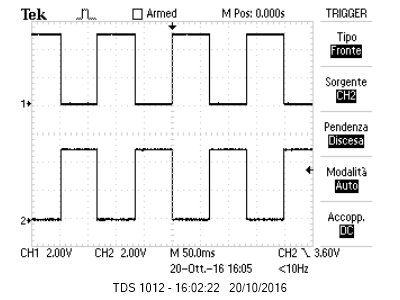
\includegraphics[scale=0.7]{not.png} 
\caption{Circuito NOT.} 
\end{figure} 


\paragraph{Misura dei tempi di transizione di $V_{out}$.}
Le misure dei tempi di transizione effettuate con l'oscilloscopio sono riportate in tabella \ref{tempi1}.
Nella fase di salita si passa da saturazione a interdizione.

\begin{table}[!htb]\centering
\begin{tabular}{|c|c|c|}
\hline 
• & Salita & Discesa \\ 
\hline 
Ritardo & $(8.7\pm0.2)\, \mu s$ & $(244\pm8) \, ns$ \\ 
\hline 
Transizione & $(1.68\pm0.04)\, \mu s$ & $(224\pm8) \, ns$ \\ 
\hline 
\end{tabular} 
\caption{Misure dei tempi.} 
\label{tempi1}
\end{table}

\paragraph{Discussione sui tempi di transizione di $ V_{out}$.}
I tempi di transizione sono dovuti alla capacità della regione di svuotamento delle due giunzioni che si comporta come un condensatore, dove la larghezza della regione è propio la distanza tra le lastre. \\
Nel modello h-ibrido tale capacità può essere aggiunta in parallelo alle resistenze dinamiche delle giunzioni. Nella situazione di interdizione la regione di svuotamento è grande e dunque la capacitò associata è piccola così come è piccolo il tempo di scarica del circuito RC associato. In zona di saturazione la capacità associata è piccola così come il tempo di salita. 
\\Questo spiega perchè i tempi (di ritardo e di transizione) associati alla discesa sono minori di quelli associati alla salita.

\paragraph{Cambiamento della resistenza $R_2$.}
La resistenza $R_2$ è il parallelo alla resistenza dinamica della giunzione base emettitore ($h_{ie}$), utilizzando la formula di Shockley questa può essere stimata come: $h_ie = \frac{\eta V_T}{I_C} \sim 1 \, k \Omega$. \\
La resistenza che compare nella stima della costante di tempo è il parallelo tra $R_2$ e $h_{ie}$, dunque per ottenere della variazioni nel tempo caratteristico bisogna scegliere resistenze $R_2$ dello stesso ordine di grandezza della resistenza dinamica. \\
Togliendo la resistenza i tempi non cambiano significativamente questo perchè aggiungere una resistenza di $100 \, k\Omega$ in parallelo a una da $\ k\Omega$ non cambia la resistenza totale. Si riportano qui di seguito le misure dei tempi (\ref{tempi2}) per una resistenza $R_2 = 4.7 k\Omega$.

Nella figura \ref{condensatore}, si vede una chiara curva esponenziale dovuta alla scarica di un condensatore.\\

\begin{figure}[!htb]
  \centering
  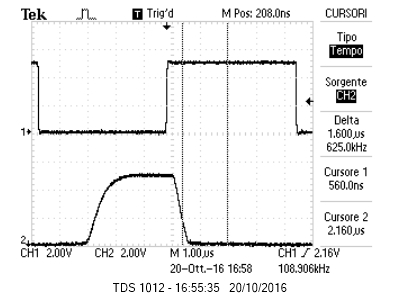
\includegraphics[scale=0.7]{condensatore.png} 
\caption{Circuito logico NOT.} \label{condensatore}
\end{figure} 

Dalla figura \ref{condensatore} si vedono anche qualitativamente le presenza dei tempi di ritardo e di transione.\\

\begin{table}[!htb]\centering
\begin{tabular}{|c|c|c|}
\hline 
• & Salita & Discesa \\ 
\hline 
Ritardo & $(2.90\pm0.08)\, \mu s$ & $(280\pm10) \, ns$ \\ 
\hline 
Transizione & $(940\pm8)\,ns$ & $(220\pm10) \, ns$ \\ 
\hline 
\end{tabular} 
\caption{Misure dei tempi con $R_2 = 4.7 \, k\Omega$.} \label{tempi2}
\end{table}

Diminuire la resistenza dovrebbe (secondo il modello prima esposto) abbassare i tempi sia di salita che di discesa. I tempi di Discesa rimangono tuttavia abbastanza stabili.\\
E' necessario del tempo perchè la corrente di base della fase di saturazione si annulli per passare il fase di interdizione, diminuire la resistenza $R_2$ diminuisce la corrente di base e quindi anche il tempo associato alla salita (passaggio in interdizione).

\paragraph{Verifica funzionamento del circuito.}
Si è verificato che le prime distorsioni apprezzabili dal comportamemento ideale del circuito si verificano alla frequenza di $20 \, kHz$.

\end{document} 